\section{La température qui monte (3 points)}\label{ex:fusion}

Dans un récipient qui contient de l'eau, on a placé un thermomètre. On a relevé la température de l'eau toutes les 10 min.

\begin{center}
	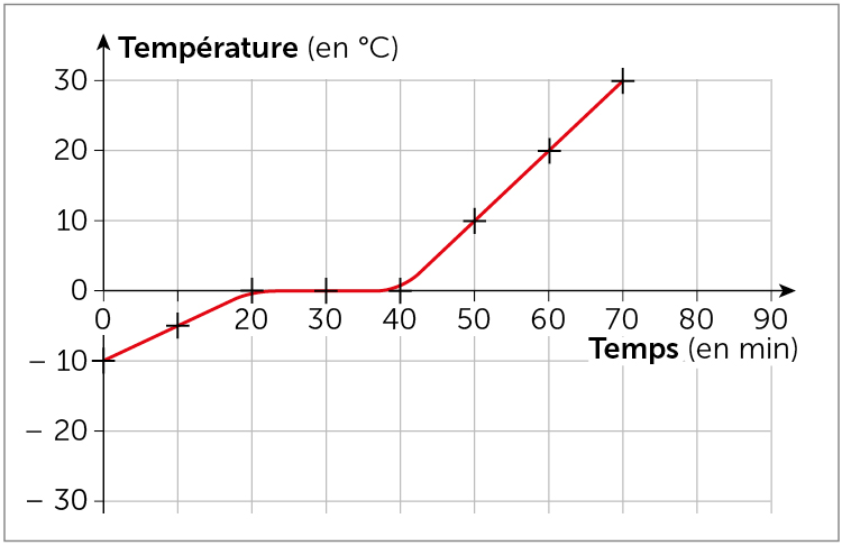
\includegraphics[scale=0.4]{./img/courbe}
\end{center}

\begin{questions}
	\question[1] Quel est l'état de l'eau après 10 minutes ? Après 60 minutes ?
	\begin{solution}
		Après 10 min, la température est inférieure à 0°C donc l'eau est solide. Après 60 min, le température est supérieure à 0°C, donc l'eau est liquide.
	\end{solution}
	
	\question[1] Combien de temps a duré le changement d'état ?
	\begin{solution}
		Sur la courbe, il y a un palier de température à 0°C entre 20 et 40 min, donc le changement d'état a duré 20 min.
	\end{solution}
	
	\question[1] A quel instant n'y a-t-il plus d'eau solide dans le récipient. 
	\begin{solution}
		Il n'y a aura plus d'eau solide dans le récipient à la fin du changement d'état, donc à 40 min.
	\end{solution}
\end{questions}